\documentclass[final]{beamer}
\mode<presentation>
{
  \usetheme{Szeged}
\usecolortheme{crane}
}


\usepackage{times}
\usepackage{multicol}
\usepackage{amsmath,amssymb,amsthm}

\newtheorem{alg}{Algorithm}

\newcommand{\argmax}{\text{argmax}}
\usepackage{float, caption, subcaption}
\usepackage[english]{babel}
\usepackage[latin1]{inputenc}
\usepackage{beamerposter}  % e.g. custom size poster
  \title[Hangman]{{\veryHuge An Optimization Layer for Distributed Matrix Computations }}
  \author[Schramm \& Weitz]{{\Large Jonah Brown Cohen, Tselil Schramm, and Ben Weitz}}
\date{}

  \begin{document}
{\large
  \begin{frame}{} 

\maketitle

\vspace{-3cm}
\begin{center}
\begin{columns}[t]
\begin{column}{0.32\textwidth}

%----------------------------------------------------------------------------------

    \begin{block}{\huge Motivation}
\vspace{.5cm}

\begin{itemize}
\item Big data companies like Facebook, Netlix, or Google perform large-scale distributed matrix computations
\begin{itemize} {\large
\item Computations experience {\bf trade-offs} in accuracy vs. time or money. 
\begin{center}
\begin{figure}
\fbox{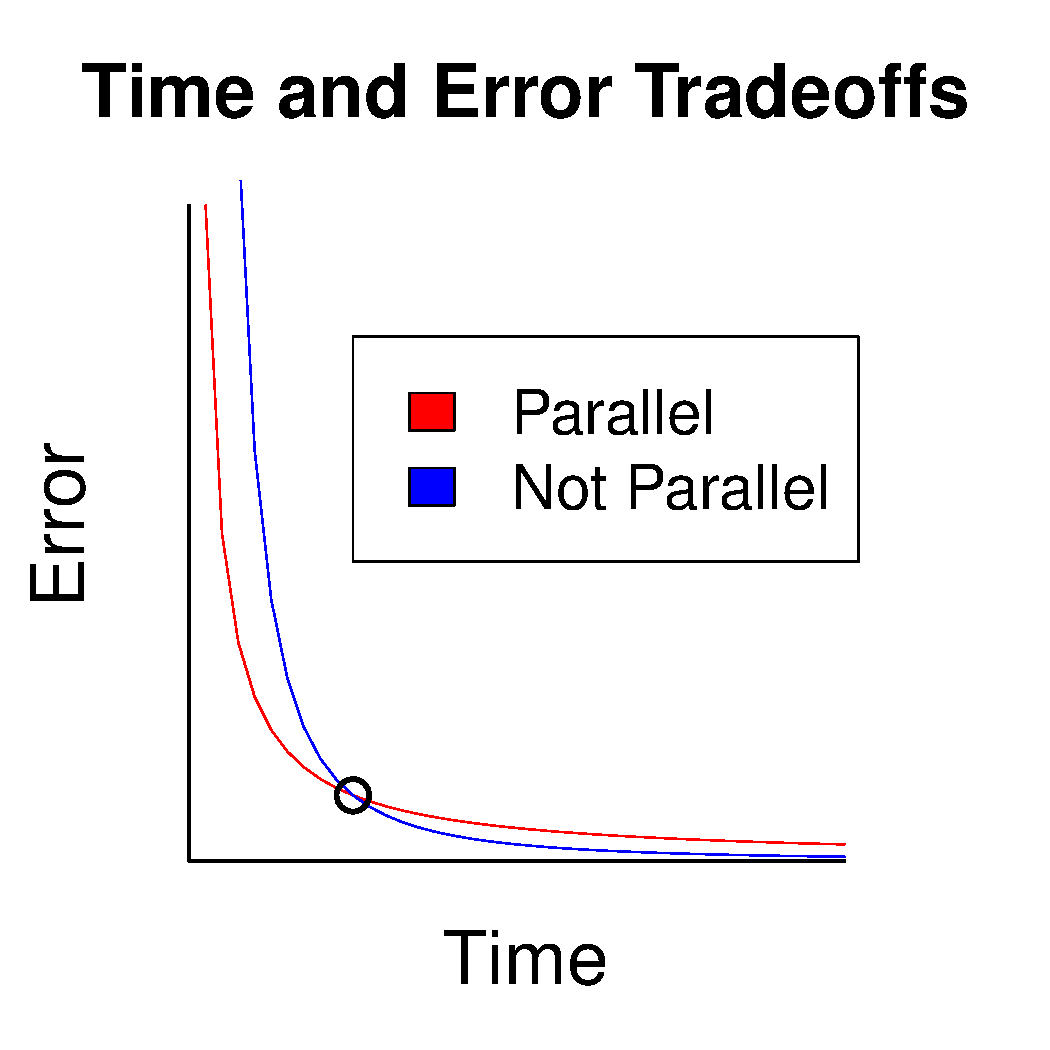
\includegraphics[width=0.35\textwidth]
{Motivations.pdf}}
\end{figure}
\end{center}
\item Human operators manually tweak parameters and partitioning
\item Humans are prone to error and costly to hire!
}
\end{itemize}
\item Solution: Build an optimization layer to automatically tweak and manage these computations
\begin{itemize} {\large 
\item Learn to adjust parameters from past computations
\item Incoming jobs come with budgets of time or accuracy that must be met
}
\end{itemize}
\end{itemize}

\end{block}

    \begin{block}{\huge Objective}
\vspace{.4cm}
\begin{itemize}
\item {\bf \large Create an optimizer that automatically picks algorithm parameters and the degree of data partitioning to meet budget specifications}
\end{itemize}

\vspace{.5cm}

\end{block}

\vspace{1.2cm}

    \begin{block}{\huge Framework}
\vspace{.5cm}
\begin{itemize}
\item Optimizer built on Python
\item Interfaces with matrix algorithms implemented in SparkR or MLBase
\item Optimizer interfaces directly with algorithms, all parameters hidden from user
\end{itemize}    
\begin{center}
\begin{figure}
\fbox{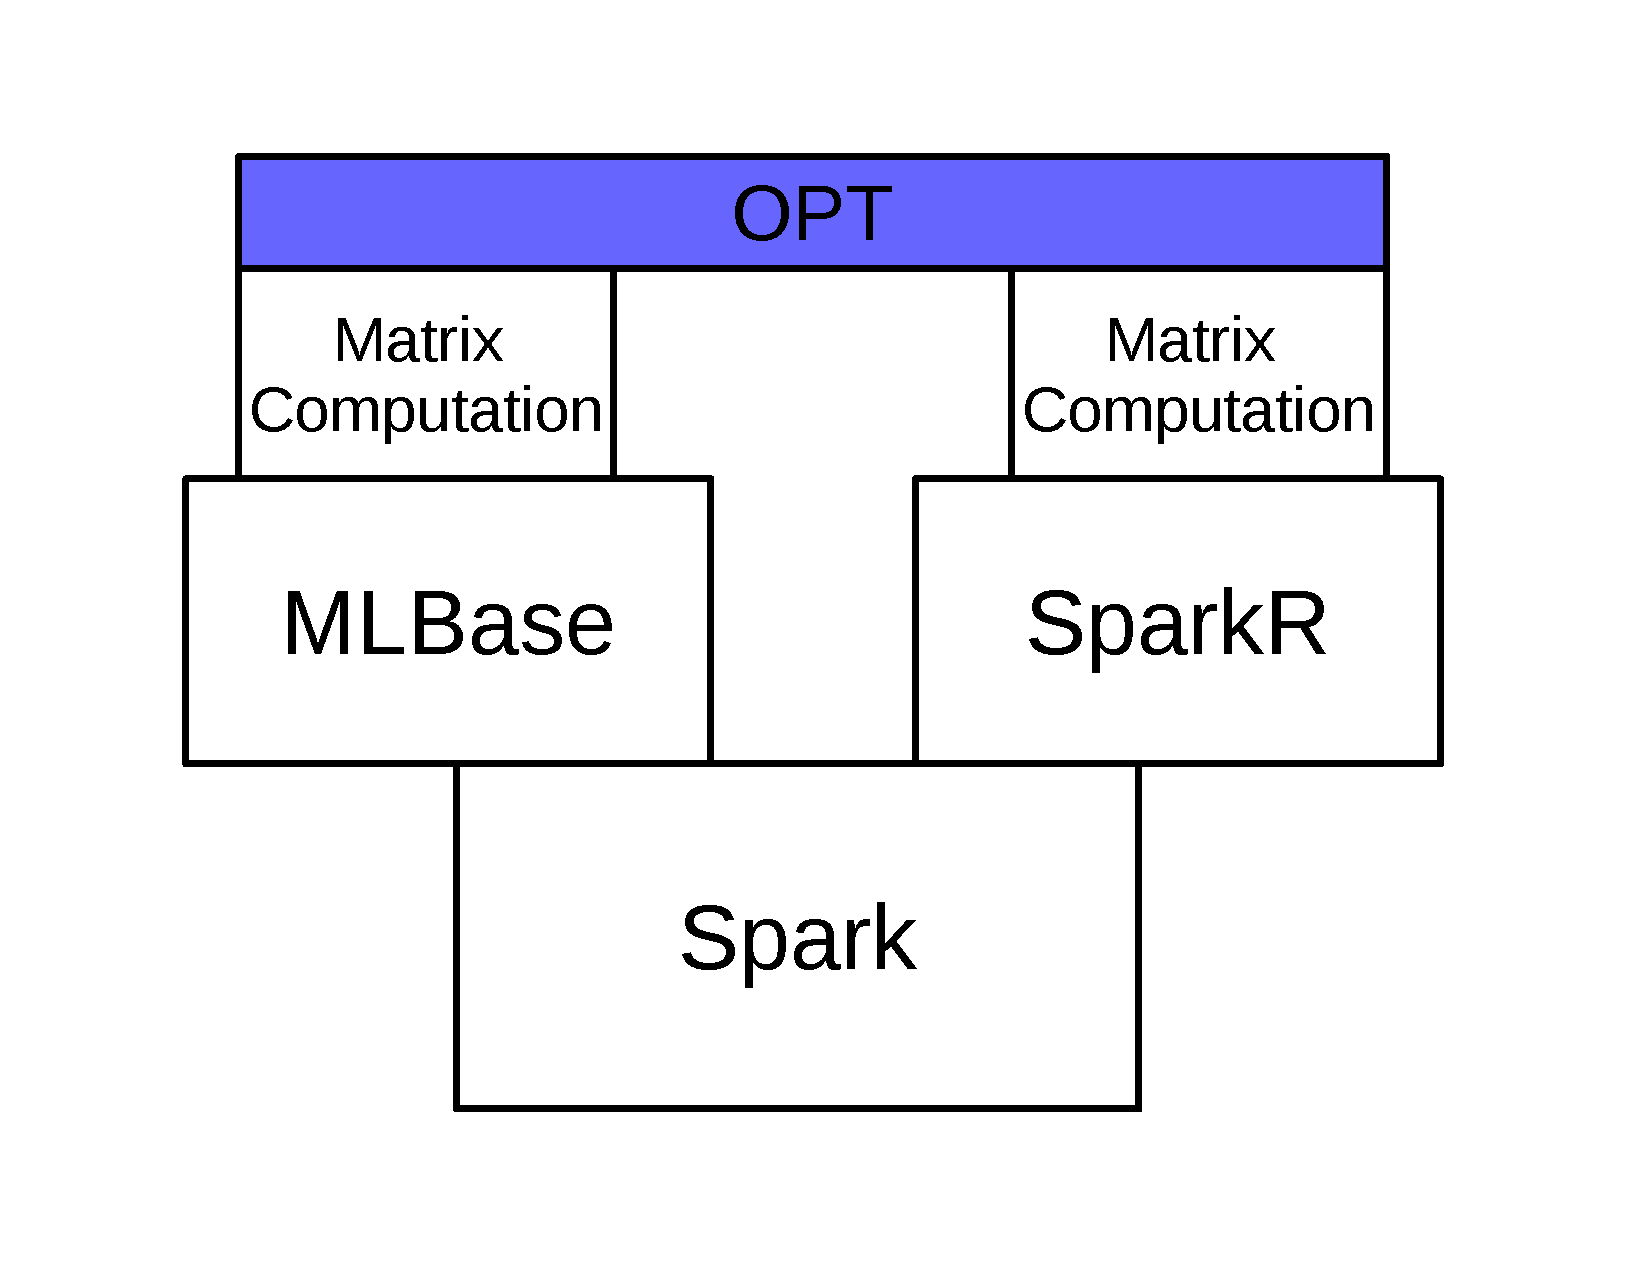
\includegraphics[width=0.5\textwidth]
{SysDiagram.pdf}}
\end{figure}
\end{center}
\end{block}

%----------------------------------------------------------------------------------

\vspace{1.2cm}

   
\end{column}

\begin{column}{0.32\textwidth}
 
    \begin{block}{\huge Optimizer Design}
\vspace{.5cm}

\begin{itemize}
\item Architecture-independent
\begin{itemize} {\large
\item Chooses parameters based on statistics from prior jobs
\item sdflksad
}
\end{itemize}

\item Adaptive
\begin{itemize} {\large
\item sdfad 
\item sdf 
}
\end{itemize}

\item Local-optimum Avoiding
\begin{itemize} {\large
\item sdfad 
\item sdf }
\end{itemize}
\end{itemize}

\begin{center}
\begin{figure}
\fbox{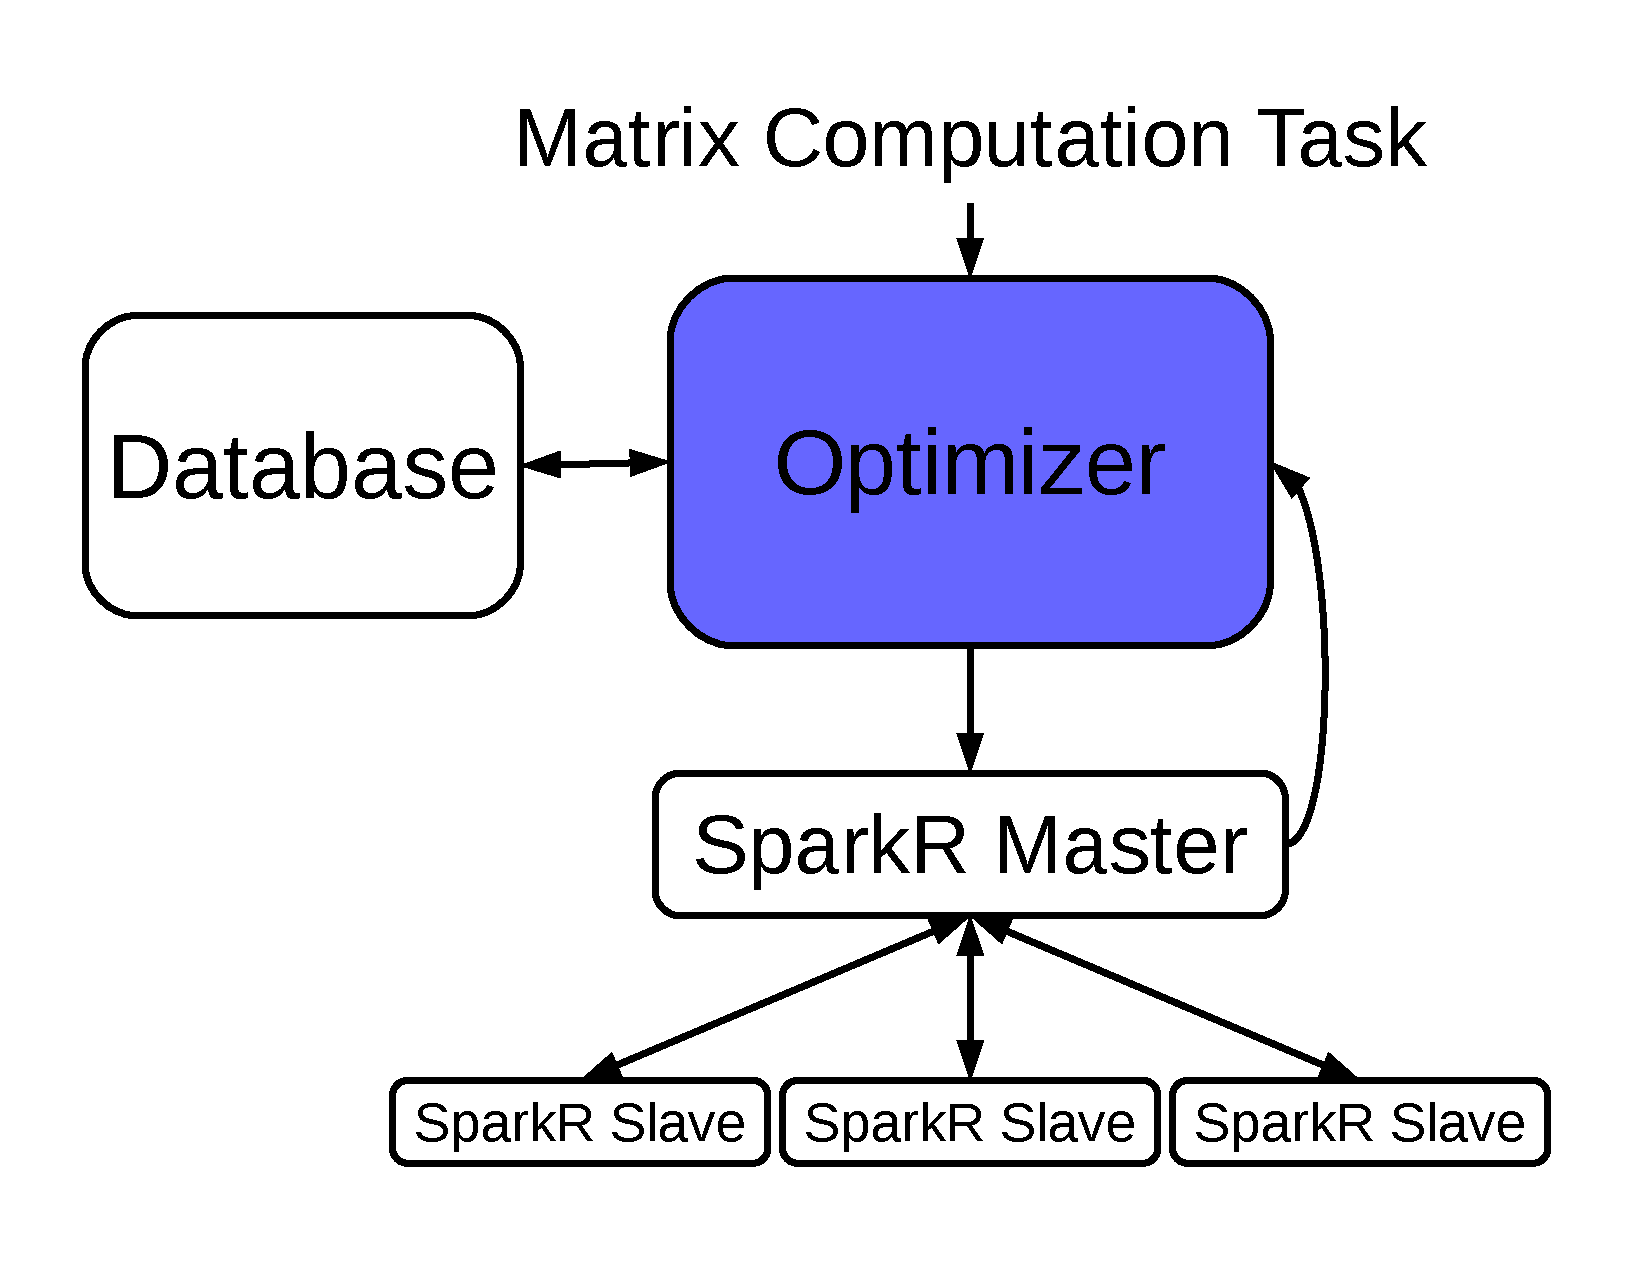
\includegraphics[width=0.7\textwidth]
{BoxDiagram.pdf}}
\end{figure}
\end{center}


\end{block}

\vspace{1.5cm}

    \begin{block}{\huge Implementation}

\vspace{.5cm}
\begin{itemize}
\item The words chosen by the adversary are hard,
\begin{itemize}{\large
\item But once you know theyre difficult it's easy to adjust.}
\end{itemize}
\item Top 12 words {\color{orange}(probability of losing in 6 turns)}:
\end{itemize}

    \end{block}


\end{column}

\begin{column}{0.32\textwidth}

       \begin{block}{\huge Evaluation}

\vspace{1cm}
{\Large Tested on Synthetic and Real-world Data}
\begin{itemize}
\item Gaussian Random Matrices
\begin{itemize} {\large
\item Trained on eight random matrices and tested on a ninth}
\begin{figure}
	\begin{subfigure}[b]{.45\textwidth}
\begin{center}
		\fbox{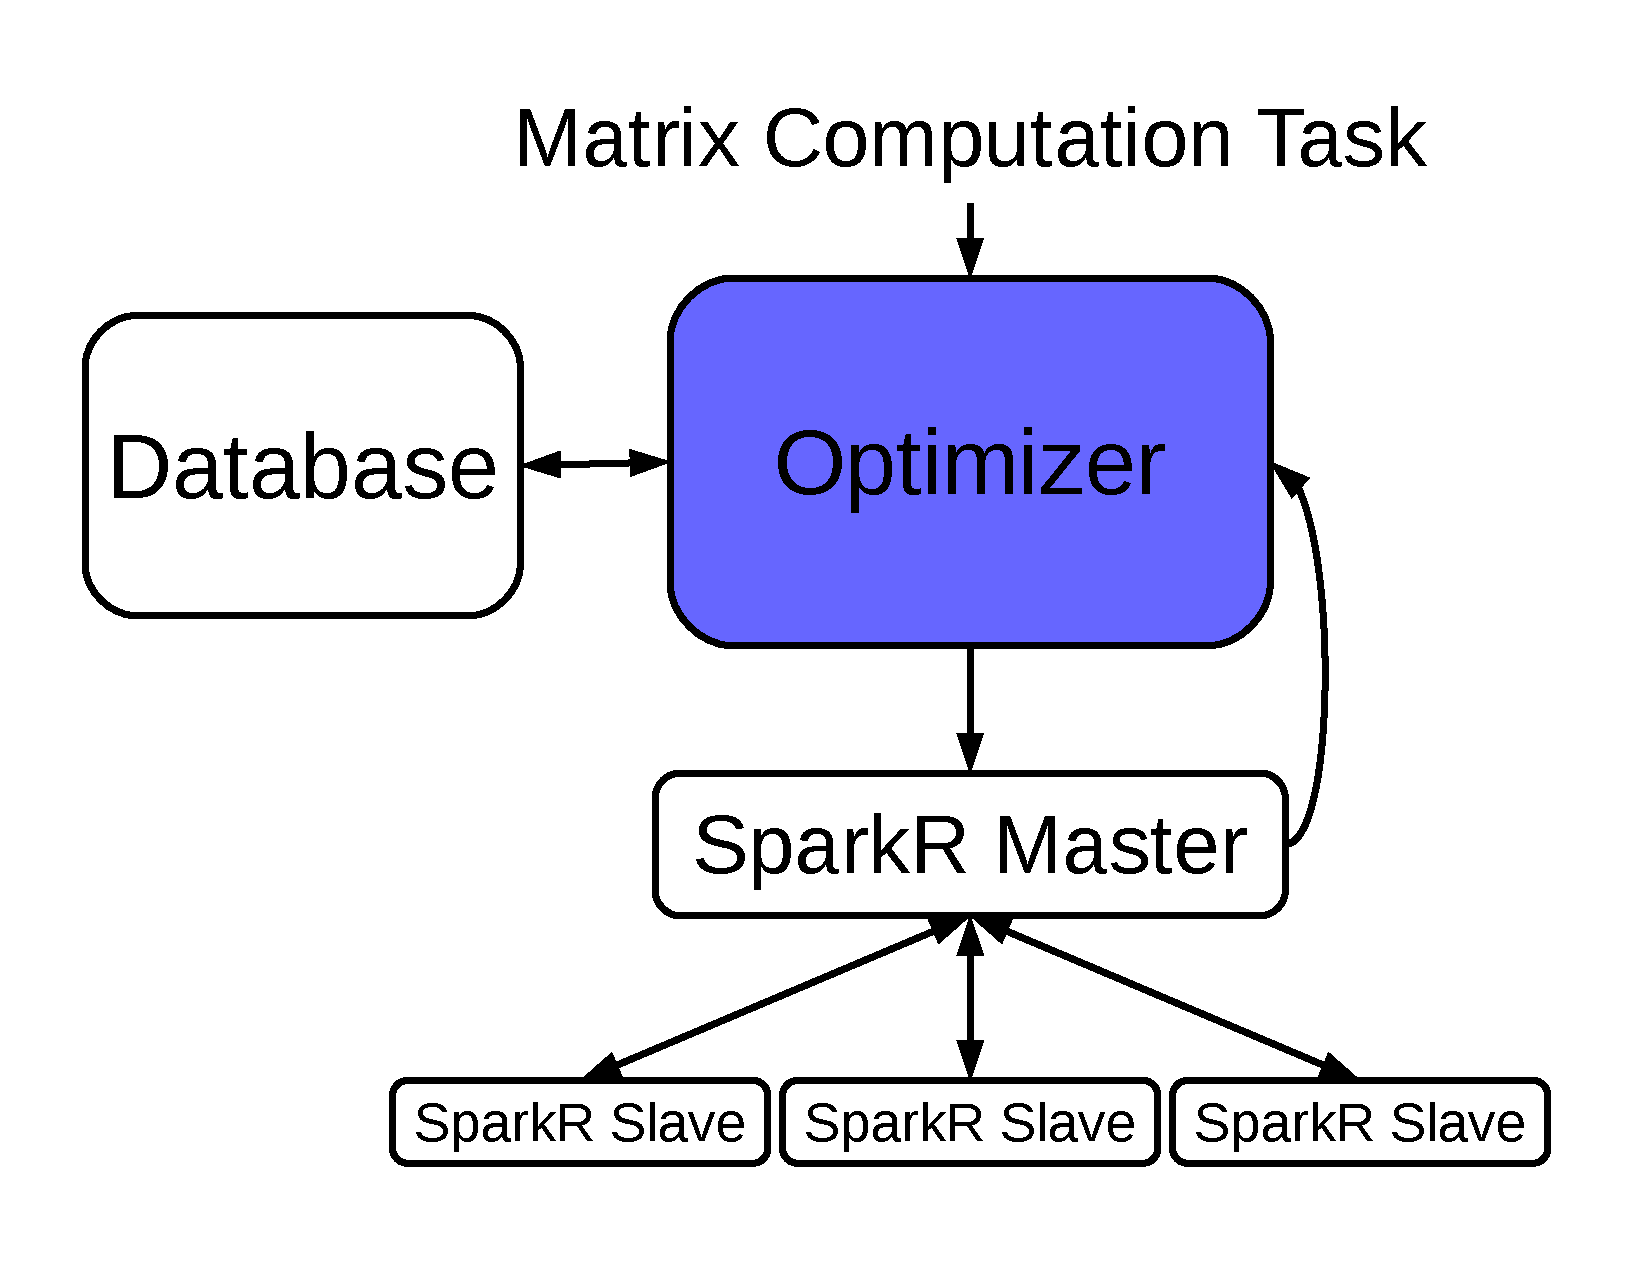
\includegraphics[width=\textwidth]{BoxDiagram.pdf}}
		\caption{AIC values.}
\end{center}
	\end{subfigure}
\hspace{1cm}
	\begin{subfigure}[b]{.45\textwidth}
\begin{center}
		\fbox{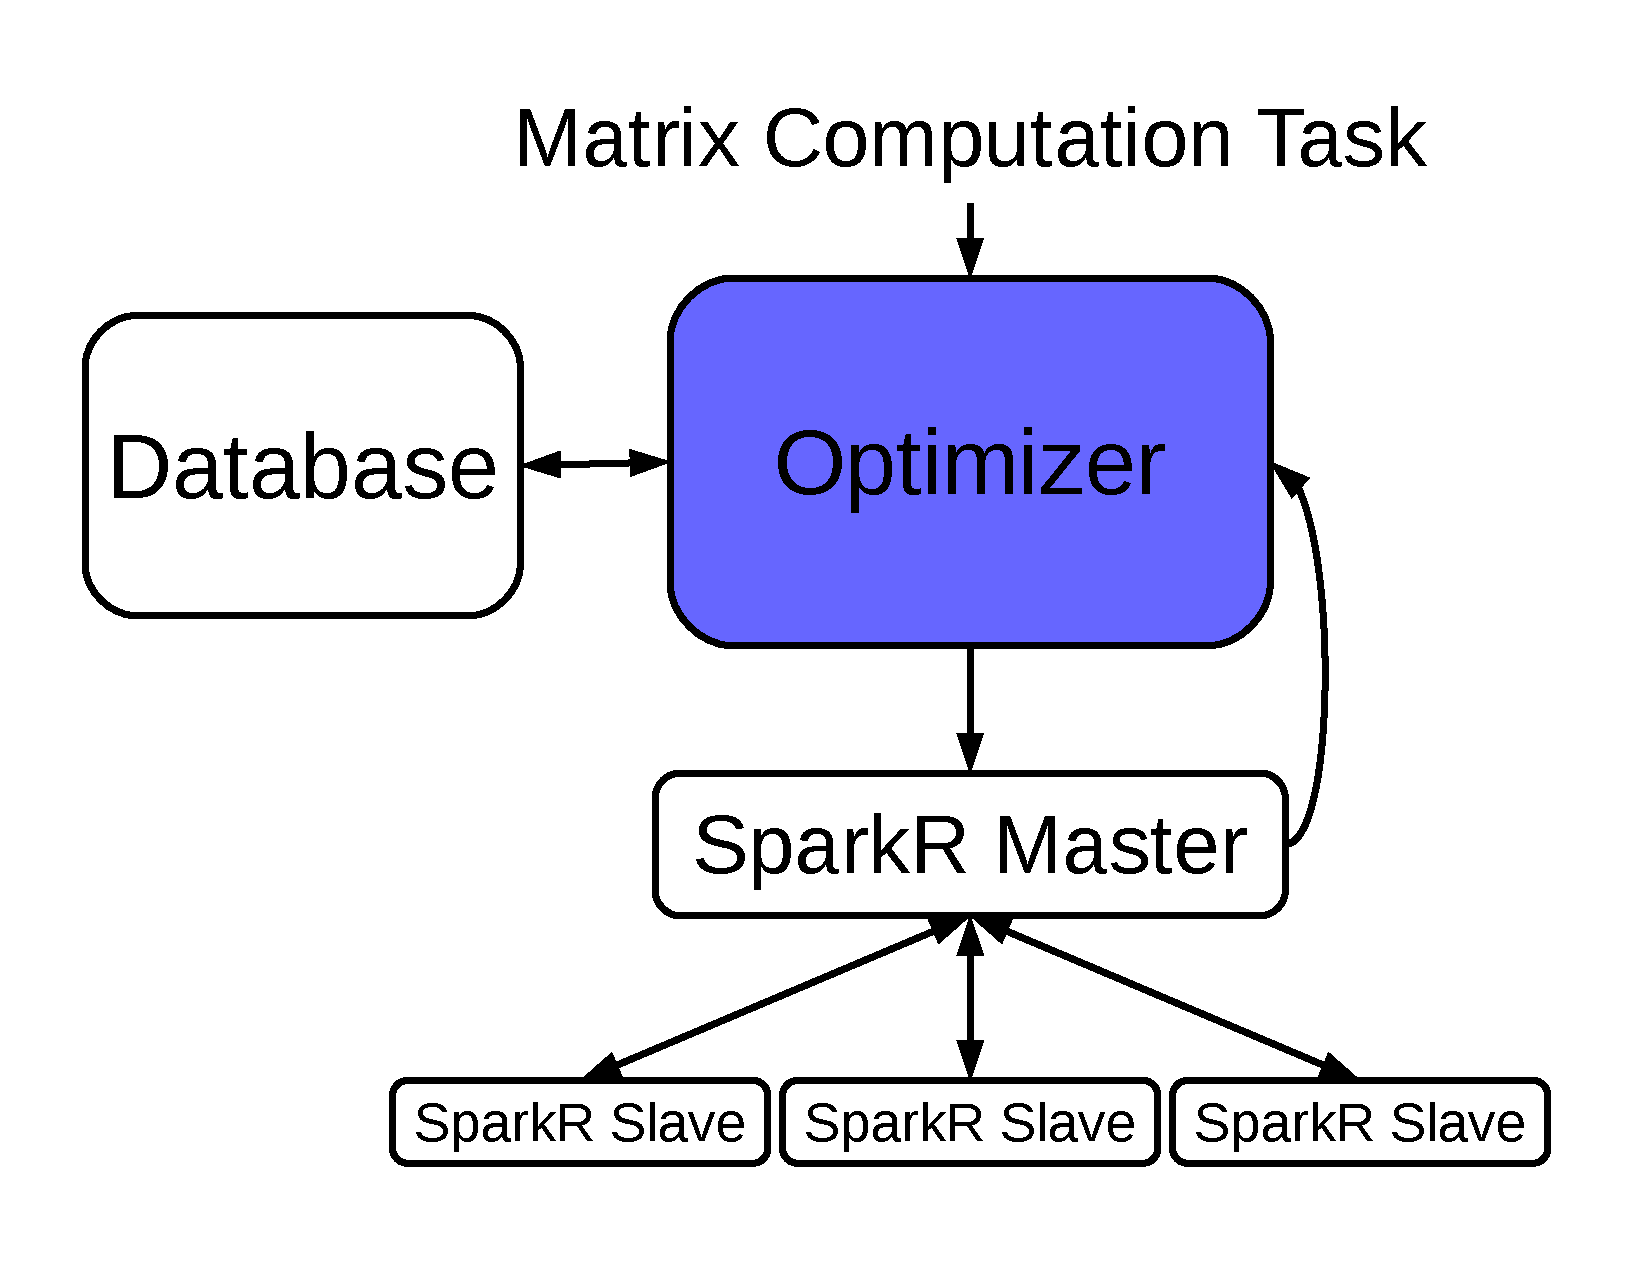
\includegraphics[width=\textwidth]{BoxDiagram.pdf}}
		\caption{BIC values.}
\end{center}
	\end{subfigure}
\hfill
	\caption{Plots of AIC and BIC Values against the Memory Parameter for a Dictionary Player with True Memory $2$}	
\end{figure}
\end{itemize}

\item MovieLens 10M Dataset
\begin{itemize} {\large
\item Partitioned dataset into 7 parts
\item Trained on all but one partition and tested on the remainder}
\begin{figure}
	\begin{subfigure}[b]{.45\textwidth}
\begin{center}
		\fbox{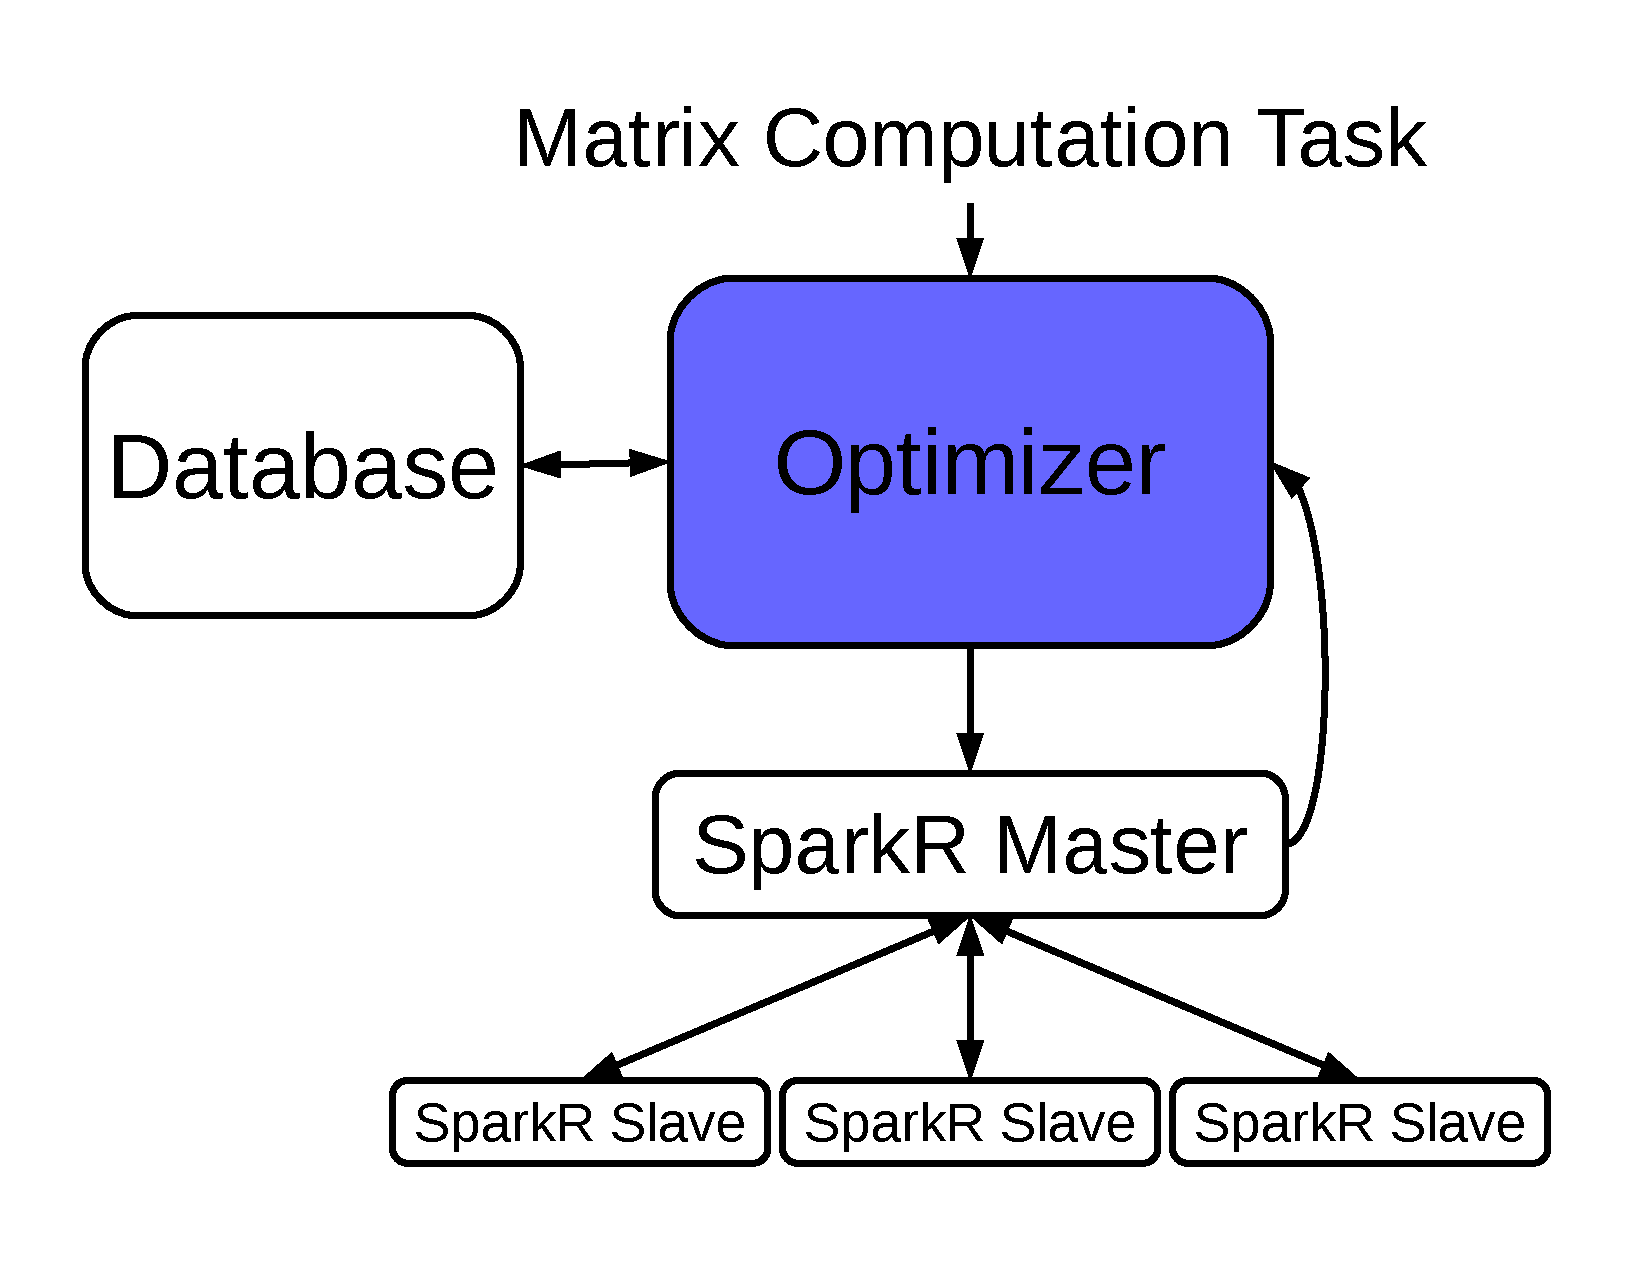
\includegraphics[width=\textwidth]{BoxDiagram.pdf}}
		\caption{AIC values.}
\end{center}
	\end{subfigure}
\hspace{1cm}
	\begin{subfigure}[b]{.45\textwidth}
\begin{center}
		\fbox{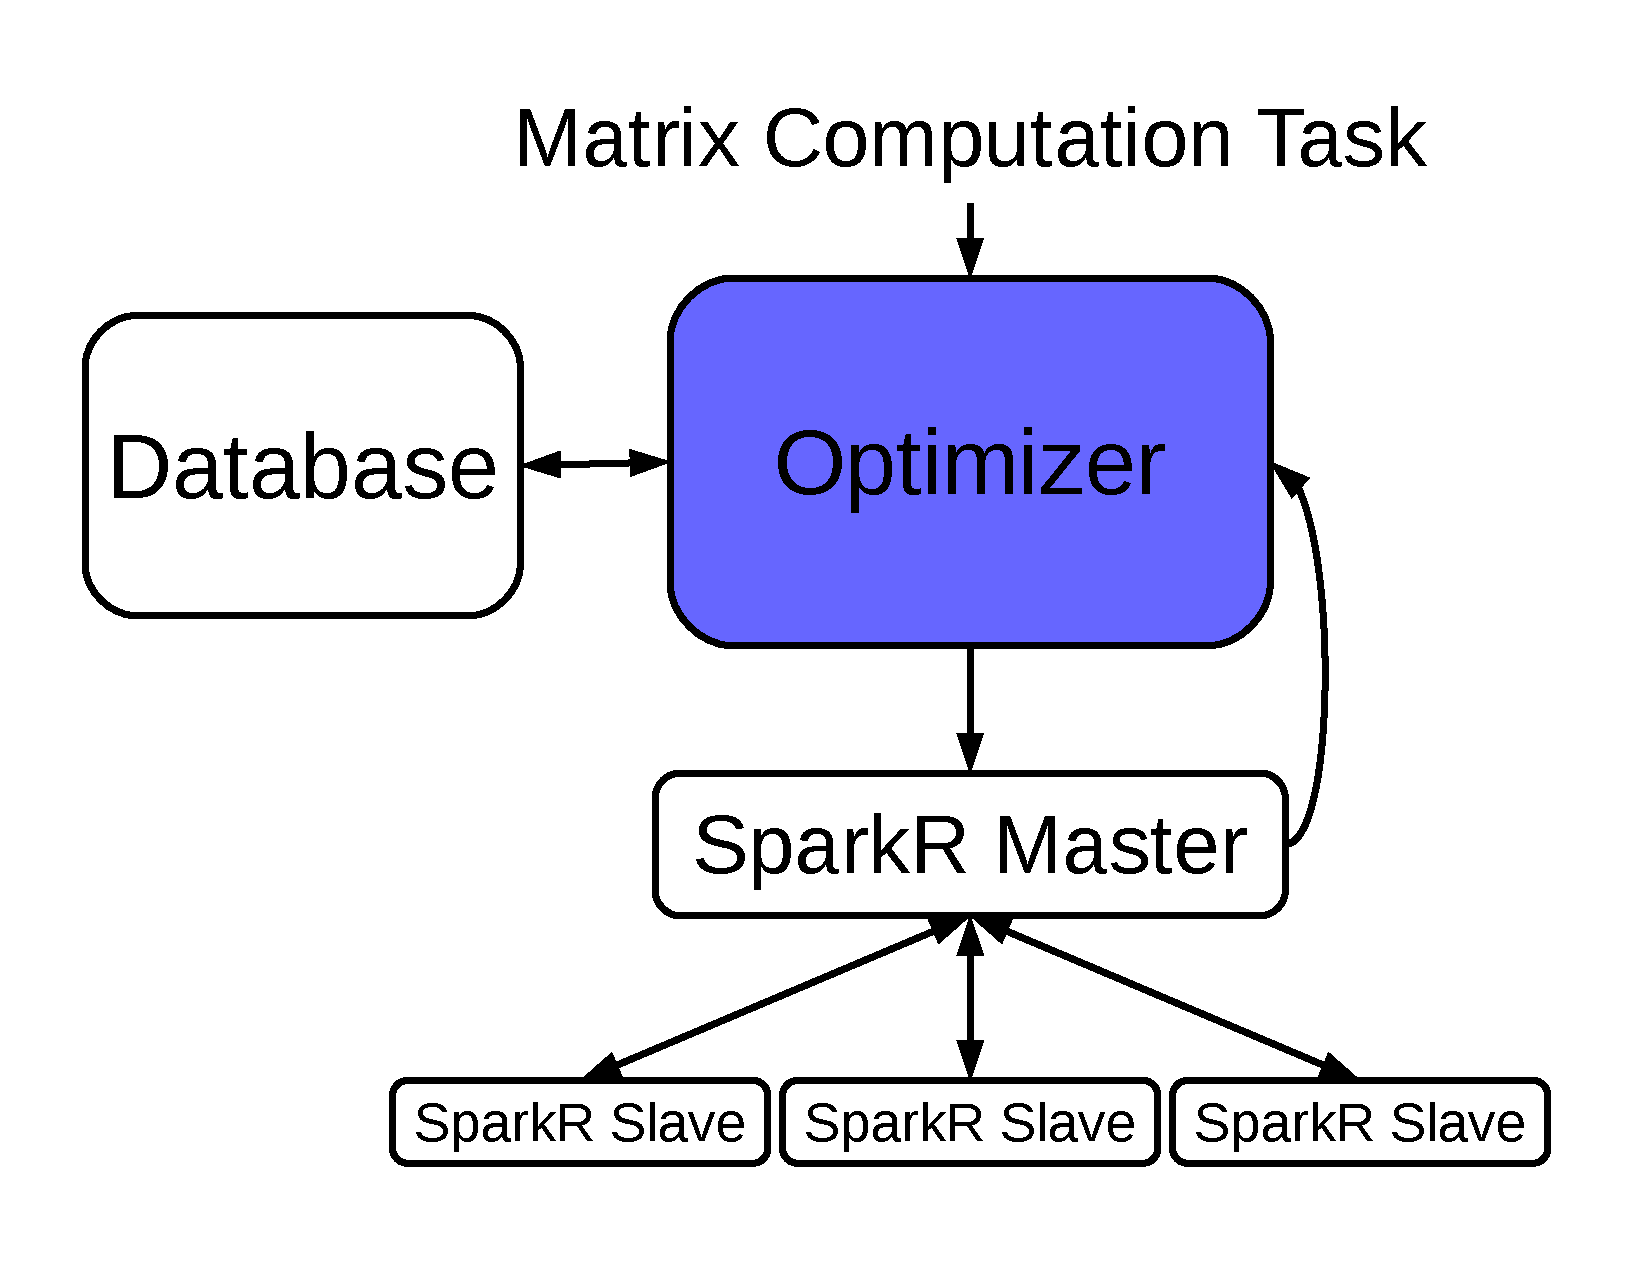
\includegraphics[width=\textwidth]{BoxDiagram.pdf}}
		\caption{BIC values.}
\end{center}
	\end{subfigure}
\hfill
	\caption{Plots of AIC and BIC Values against the Memory Parameter for a Dictionary Player with True Memory $2$}	
\end{figure}
\end{itemize}
\item Optimizer performs as well as manually setting the parameter!
\end{itemize}

\vspace{1cm}
    \end{block}

\vspace{1.5cm}

    \begin{block}{\huge Future Work}
\begin{itemize}
\item Optimize over space of algorithms in addition to space of parameters
\item Avoid RAM bottlenecks by distributing collect step
\item Handle novel or different jobs
\end{itemize}
\vspace{.5cm}
    \end{block}

\vspace{1.5cm}

    \begin{block}{\huge Acknowledgements}
We would like to thank:
\begin{itemize}
\item Shivaram Venkataraman, Ameet Talwalkar, Prof. Anthony Joseph, and Prof. John Kubiatowicz
\item UC Berkeley and the NSF for providing funds and resources.
\end{itemize}
    \end{block}
\end{column}

\end{columns}
\end{center}
\vspace{1.5cm}
  \end{frame}
  \end{document}